\section{Method}
\label{sec:method}

\subsection{Style-Controlled Rewriting}
\label{sec:rewriting}

We isolate the effect of individual style attributes on judge scores by generating text pairs that differ along exactly one style axis while holding content fixed---a single-axis intervention design that enables per-axis causal attribution rather than aggregate style sensitivity measurement.
For each text, an instruction-tuned LLM (Qwen3-32B) classifies its current style along the target axis (e.g., formal vs.\ casual via binary classification).
It then rewrites the text toward the opposite pole (temperature 0.7, selected to balance diversity with coherence in pilot experiments) according to an axis-specific prompt (Appendix~\ref{app:rewriting_prompts}).
This produces a dataset balanced across both directions at the dataset level: texts detected as formal are rewritten to casual, and vice versa.
Each operation approximates a binary intervention on a single style variable while all other axes remain fixed (Section~\ref{sec:causal_framework}; Appendix~\ref{app:cross_axis_contamination}).
To control for rewriting artifact bias---the possibility that the judge prefers original text over any rewrite regardless of style---we additionally generate a same-style double-rewrite for each text (e.g., formal $\to$ formal) to form an original-vs-double-rewrite control pair, following the RATE bias correction protocol \citep{reber2025rate}.

\subsection{Content Preservation Verification}
\label{sec:nli_gate}

Style-controlled rewriting risks altering semantic content, which would confound the style effect with a content quality effect (the $R \to Q$ path in Figure~\ref{fig:dag}).
To block this path, we apply a natural language inference (NLI) gate using DeBERTa-v3-large fine-tuned on MNLI \citep{williams2018broad} with an entailment threshold of 0.90, selected as the threshold above which NLI performance plateaus (Appendix~\ref{app:nli_sweep}).
For axes that preserve information density (formality, register), we apply standard bidirectional entailment: both NLI(original $\to$ rewrite) and NLI(rewrite $\to$ original) must exceed this value.
For axes that inherently change information density (e.g., verbosity), bidirectional verification is inappropriate---expansion necessarily introduces new content that the original cannot entail.
We instead apply direction-aware verification: for expansions, only backward entailment (rewrite entails original); for compressions, only forward entailment (original entails rewrite).
This recovered verbosity from 65\% to 86\% pass rate without inflating the effect estimate; for formality, strict bidirectional gating is necessary (Appendix~\ref{app:gate_validation}).
This gating mechanism provides filtering-based confounder control \citep{veitch2020adapting} by ensuring that retained pairs differ only in style, not in content quality (validated by human annotation; \S\ref{sec:nli_validation}).
BERTScore serves as a supplementary monitor but does not participate in gating.

\begin{figure}[t]
\centering
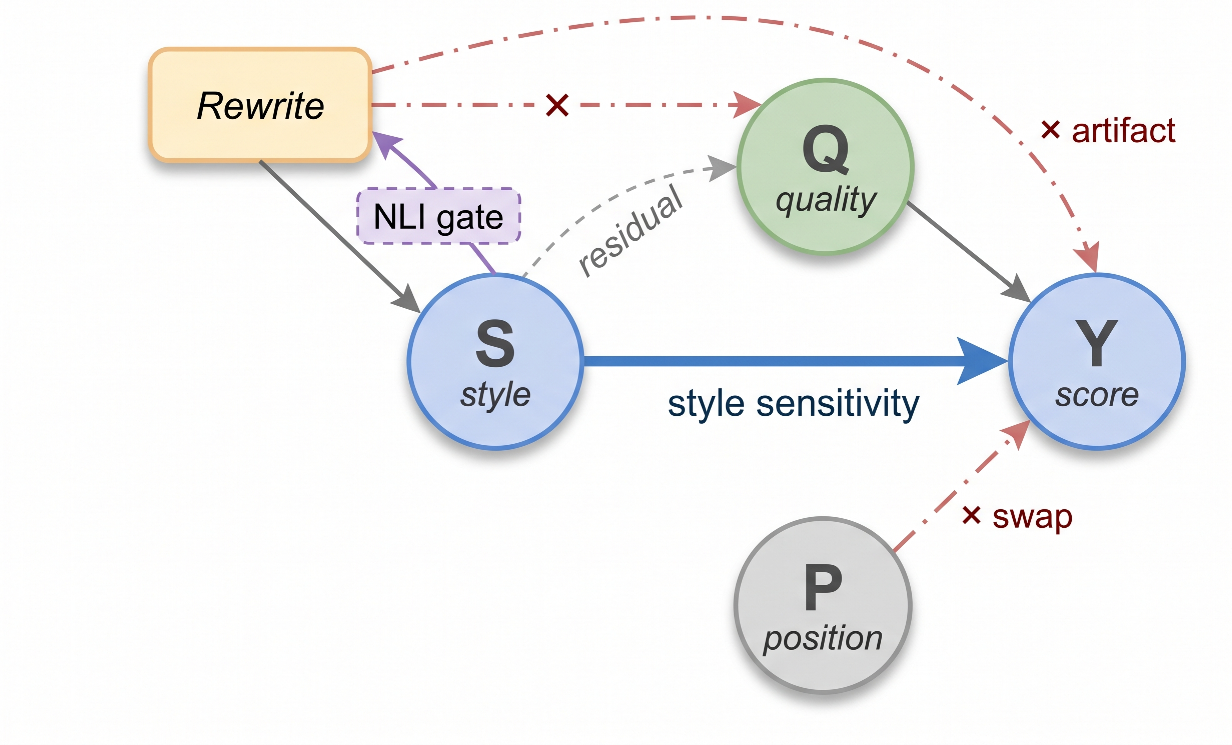
\includegraphics[width=\columnwidth]{figures/dag_diagram.pdf}
\caption{Assumed data-generating process (design rationale, not a claim of perfect identification). The rewriting mechanism $R$ targets style $S$ but may inadvertently alter content quality $Q$ (dash-dot, blocked by NLI gate) or introduce rewriting artifacts ($R \to Y$, blocked by double-rewrite control). Position bias $P \to Y$ is controlled by order swapping. The dashed $S \to Q$ path represents residual confounding (Limitations). $Y$: judge score.}
\label{fig:dag}
\end{figure}

\subsection{Measurement Protocol}
\label{sec:measurement}

Each pair that passes the NLI gate is evaluated by four target judges---GPT-4o (\texttt{gpt-4o-2024-08-06}), Qwen3-32B, Llama-3.3-70B, and Gemini-2.5-Flash---under two complementary scoring modes.
In Likert mode, the judge assigns an integer score from 1 to 10 for overall quality to each text independently; the coarse integer scale is typical of deployed evaluation systems but limits measurement resolution for subtle effects.
In pairwise mode, the judge receives both texts as candidates A and B and makes a forced choice of which response is better, eliminating anchoring effects inherent in absolute rating.

To control for position bias, each pairwise comparison is evaluated twice with the presentation order swapped, which produces $n_{\text{pairs}} \times 2$ observations.
We apply two analysis strategies to these data.
For the nonparametric sign test, we retain only \emph{consistent} pairs where the judge selected the same text in both orderings.
For the Bradley-Terry model, we use all observations including inconsistent pairs, as the model naturally accommodates noise in individual comparisons.
The BT model assumes a single latent quality dimension; per-axis GEE decomposition (\S\ref{sec:direction}) complements this by separating style-specific from quality-correlated components.

\subsection{Experimental Setup}
\label{sec:setup}

We evaluate on LLMBar \citep{zeng2023llmbar}, a benchmark of $n = 100$ instruction-response pairs spanning diverse task types, designed to test LLM judges' ability to distinguish response quality with human-verified quality labels.
LLMBar is well-suited for style sensitivity detection because its human-verified labels provide ground truth against which judge deviations can be measured, and its moderate size permits exhaustive pairwise evaluation with position control.
We select formality and verbosity as primary axes based on prior evidence that these are among the most commonly reported style sensitivities in LLM judges \citep{wu2023style,saito2023verbosity} (implementation details in Appendix~\ref{app:implementation}).

\subsection{Design Rationale}
\label{sec:causal_framework}

Figure~\ref{fig:dag} presents the assumed data-generating process.
CSD approximates the effect of style $S$ on judge score $Y$ while blocking confounding through content quality $Q$: the NLI gate blocks $R \to Q$, position swapping controls presentation order, and the rewrite targets a single axis.
Our approach provides interventional rather than formal causal evidence (details in Appendix~\ref{app:design_rationale}).
A tone axis pilot (assertive $\to$ hedging) did not pass NLI gating, establishing a practical scope boundary for CSD at surface-level axes (Limitations).
